%%
%% This is file `mcmthesis-demo.tex',
%% generated with the docstrip utility.
%%
%% The original source files were:
%%
%% mcmthesis.dtx  (with options: `demo')
%% 
%% -----------------------------------
%% 
%% This is a generated file.
%% 
%% Copyright (C)
%%       2010 -- 2015 by latexstudio
%%       2014 -- 2019 by Liam Huang
%%       2019 -- present by latexstudio.net
%% 
%% This work may be distributed and/or modified under the
%% conditions of the LaTeX Project Public License, either version 1.3
%% of this license or (at your option) any later version.
%% The latest version of this license is in
%%   http://www.latex-project.org/lppl.txt
%% and version 1.3 or later is part of all distributions of LaTeX
%% version 2005/12/01 or later.
%% 
%% This work has the LPPL maintenance status `maintained'.
%% 
%% The Current Maintainer of this work is latexstudio.net.
%% 
%%
%% This is file `mcmthesis-demo.tex',
%% generated with the docstrip utility.
%%
%% The original source files were:
%%
%% mcmthesis.dtx  (with options: `demo')
%%
%% -----------------------------------
%%
%% This is a generated file.
%%
%% Copyright (C)
%%       2010 -- 2015 by latexstudio
%%       2014 -- 2019 by Liam Huang
%%       2019 -- present by latexstudio.net
%%
%% This work may be distributed and/or modified under the
%% conditions of the LaTeX Project Public License, either version 1.3
%% of this license or (at your option) any later version.
%% The latest version of this license is in
%%   http://www.latex-project.org/lppl.txt
%% and version 1.3 or later is part of all distributions of LaTeX
%% version 2005/12/01 or later.
%%
%% This work has the LPPL maintenance status `maintained'.
%%
%% The Current Maintainer of this work is latexstudio.net.
%%


\documentclass{mcmthesis}
 %\documentclass[CTeX = true]{mcmthesis}  % 当使用 CTeX 套装时请注释上一行使用该行的设置
\mcmsetup{
        tcn = 2412216, problem = C,
        sheet = true, titleinsheet = true, keywordsinsheet = true,
        titlepage = false, abstract = true}

 %三款字体可以选择
 \usepackage{fontspec}%默认就用这个新罗马字体
\setmainfont{Times New Roman}
 %\usepackage{times}
 %\usepackage{newtxtext}%这个字体用不了,会报错?
 %\usepackage{palatino}

%%以下为从外部导入的宏包,非美赛latex自带
 \usepackage[UTF8, nocap]{ctex}%插入中文
 \usepackage{caption}%%新插入的,为了打印子图minipage
 \usepackage{diagbox}%%为了打印斜杆表格
 \usepackage{threeparttable}%%为了打印斜杠表格
 \usepackage{indentfirst}%%首段空格

\usepackage{lipsum}
\title{Modeling Momentum and Reversals in Tennis Matches: A Bayesian Approach with Horseshoe Prior}

\begin{document}
\begin{abstract}%%textbf加粗文本

In competitive sports, the phenomena of \textbf{momentum} and \textbf{reversals}, influenced by various historical factors, probably affect athletes' future scoring probabilities. 

Utilizing data from 31 tennis matches, we categorized multidimensional indicators into momentum and covariate factors, applying \textbf{logistic regression} within a \textbf{probabilistic framework} to model the \textbf{Bernoulli process} inherent in round-based sports events. This approach tackles the prevalent issues of \textbf{high-dimensionality} and \textbf{sparsity} in sports prediction by introducing the \textbf{horseshoe prior} for enhanced model robustness and interpretability. The horseshoe prior, outperforming conventional shrinkage methods like Lasso or Ridge, applies global and local shrinkage for noise reduction while preserving critical information. Furthermore, we adopted Enes Makalic and Daniel F. Schmidt's methodology, using \textbf{auxiliary variables} and \textbf{Pólya-gamma data augmentation} to simplify posterior updates.

\textbf{For question 1,} we initially assess match ID-1701, comparing coefficients and credible intervals to check the model's performance. Estimating all matches yields accuracy rates under MLE and horseshoe prior. We then use \textbf{moving and rolling windows strategies} for time series estimation on match ID-1701, evaluating out-of-sample model performance. We employ the probability parameter of the likelihood function as an indicator to evaluate player performance in the predicted rounds, leading to the generation of visualized images.\textbf{For question 2,} we enhance the model's \textbf{randomness} to assess tennis match predictability. Firstly, by removing momentum-related features and re-analyzing the 31 matches, we evaluate momentum's effect on predictability via accuracy rates under MLE and horseshoe prior. Secondly, using historical outcomes and treating each match point as an independent Bernoulli trial with a specific probability parameter, we build a \textbf{Beta-Bernoulli model} to investigate changes in the probability parameter's posterior mean throughout the matches.\textbf{For question 3,} we redefined the dependent variable to signify whether a reversal occurred and compared estimation accuracies under MLE and the horseshoe prior.\textbf{For question 4,} we extended the application of our model to various competitive events, demonstrating its \textbf{generalization capabilities}. 

The results indicate significant \textbf{randomness} in win rates per round in professional tennis matches. Nonetheless, historical information remains effect as even amidst challenges of high-dimensional and sparse data, appropriate \textbf{noise handling} methods can identify credible factors with predictive value. Additionally, many features in tennis matches exhibit significant heterogeneity, suggesting variability in momentum factors across different matches.  
  
\begin{keywords}
Competitive Sports; Momentum; Reversals; Bernoulli Process; Logistic Regression; Horseshoe Prior; High-Dimensionality
\end{keywords}
\end{abstract}


%目录!所有页数加载需要至少两次的简单编译,复杂编译容易报错。一次编译目录加载会是错的
\maketitle
%% Generate the Table of Contents, if it's needed.
 \tableofcontents
 \newpage
%%
%% Generate the Memorandum, if it's needed.
%% \memoto{\LaTeX{}studio}
%% \memofrom{Liam Huang}
%% \memosubject{Happy \TeX{}ing!}
%% \memodate{\today}
%% \logo{\LARGE I'm pretending to be a LOGO!}
%% \begin{memo}[Memorandum]
%%   \lipsum[1-3]
%% \end{memo}
%%
\section{Introduction}

\subsection{Background}

The 2023 Wimbledon Gentlemen’s final witnessed a significant upset, demonstrating that even players with consistently excellent performance can experience fluctuations in their level of play during a match, leading to a reversal of the advantage on the court. Commentators often attribute these fluctuations to changes in "momentum." However, in sports competitions, the sources of momentum are subjective and difficult to quantify, and the factors affecting momentum have remained elusive. Consequently, whether sporting outcomes are influenced by momentum or are inherently random has been a topic of much debate.

\subsection{Restatement of the Problem}
We possess a database containing detailed data from 31 matches at the 2023 Wimbledon Championships. Our objective is to construct a systematic model to address the following issues:

\begin{enumerate}
  \item Determine the performance of players at specific times during a match. The model should focus on serving factors while also providing a visualization of performance.
  \item Investigate whether momentum plays a role in matches and assess the randomness of success in the competition.
  \item Explore the determinants of reversals in matches. What recommendations can differences in momentum within the model offer to players?
  \item Apply the model to other categories of tennis, table tennis, and other racket sports data to assess the model's generalizability.
  \item Provide a 1 to 2-page memorandum to communicate with tennis coaches about the role of momentum in matches and offer suggestions.
\end{enumerate}

\subsection{Our Work}

Prior to addressing these questions, we developed a logistic regression model within a Bayesian framework to predict the win probability of players in tennis matches. We enhanced the model by incorporating the horseshoe prior, auxiliary variables, and Pólya-gamma data augmentation techniques and conducted a multifaceted evaluation of the model's accuracy. After constructing the model, we used it to interpret various issues. Below is the workflow diagram of our work.

\begin{figure}[ht]
  \small
  \centering
  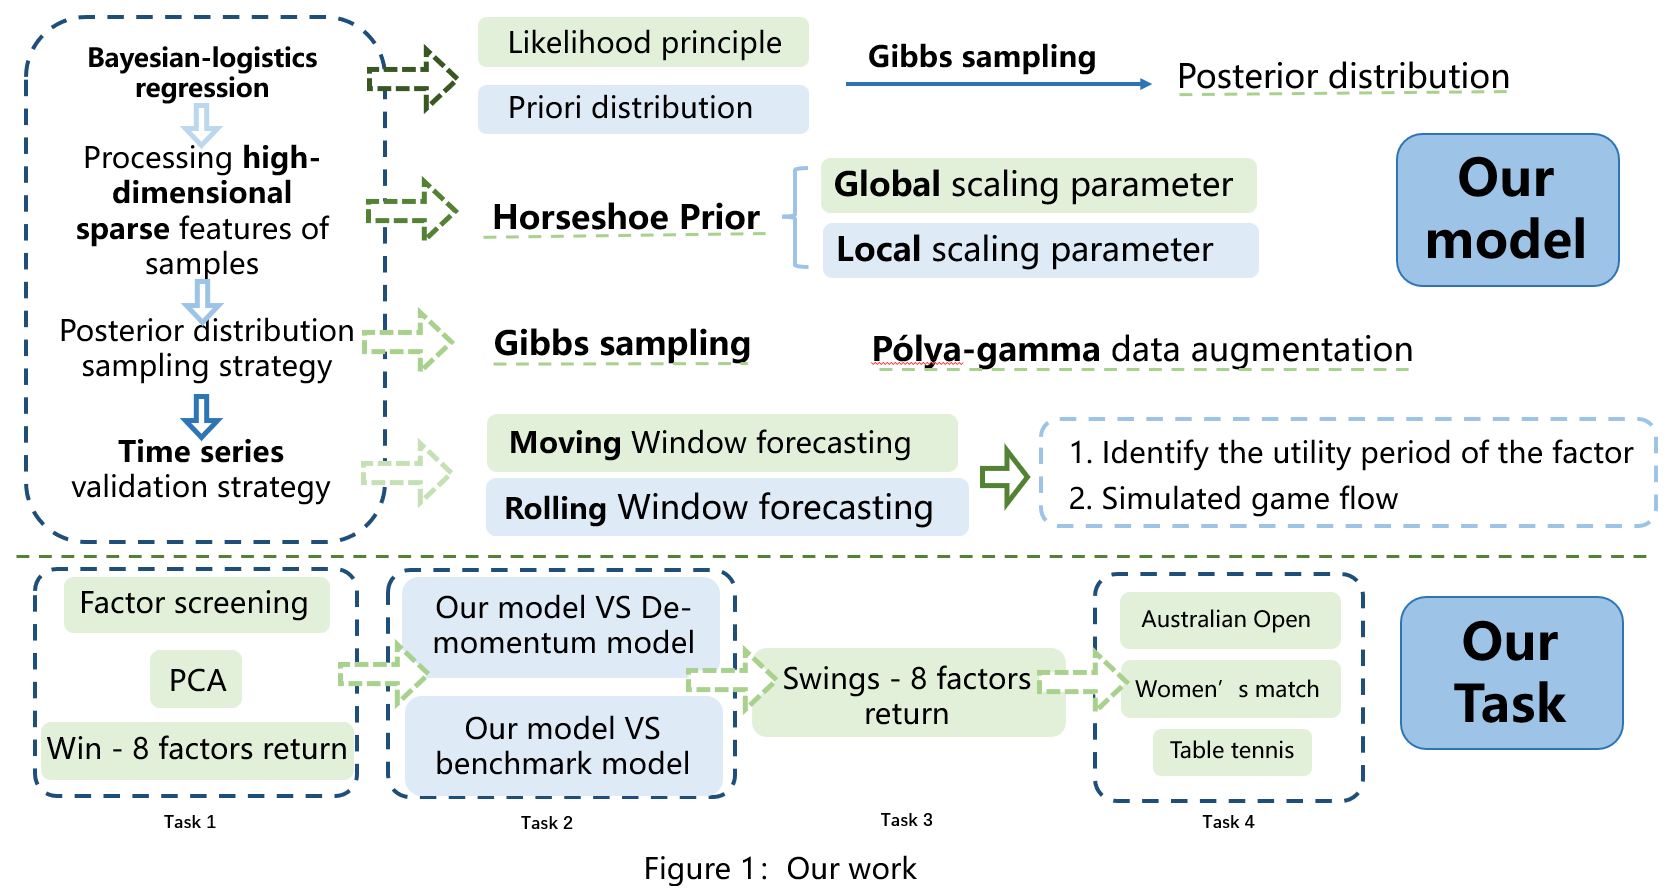
\includegraphics[width=16cm]{picture1}
\end{figure}

\newpage
\section{Model Assumptions and Notations}

Based on the problem statement, we make the following assumptions:
\begin{itemize}
  \item \textbf{Momentum Effect:}
  Momentum is assumed to be a factor influencing the probability of winning a point and is an important component of the feature vector $X_i$.
  \item \textbf{Bernoulli Process:}
  Each point-winning event is considered a Bernoulli trial, with the success probability (i.e., the probability of winning the point) denoted as $\theta$, reflecting the likelihood of a player winning a point under specific conditions.
  \item \textbf{Winning Outcome ($Y_i$):} 
  In the match, the outcome of the $i^{th}$ point is denoted as $Y_i$, where $Y_i = 1$ indicates the player won the point, and $Y_i = 0$ indicates a loss.
  \item \textbf{Feature Vector ($X_i$):}
  The feature vector $X_i$ for the $i^{th}$ point includes momentum among other key factors, aimed at capturing various elements that may influence the probability of winning a point during the match.
\end{itemize}

\section{Model Establishment}
\subsection{Bayesian Logistic Regression with Horseshoe Prior}
We have established a logistic regression model within a Bayesian framework, particularly focused on the application in sports statistics, such as predicting the win probability of players in tennis matches. For each player, each round of the match results in only two outcomes: scoring or not scoring. Hence, each round's win event is considered a Bernoulli trial with the success probability (i.e. the probability of winning the point) denoted by $\theta$, reflecting the likelihood of a player winning a point under specific conditions. The logistic regression model is chosen as it directly estimates the probability of an event's occurrence, thus predicting the win probability. Moreover, given the potential for high-dimensionality and sparsity within the model, this paper introduces the horseshoe prior to enhance the robustness and interpretability of the model. We will also discuss how to simplify the updating process of the posterior distribution by introducing auxiliary variables and employing the Pólya-gamma data augmentation method, making the model more efficient and easy to implement. The main steps of the model are provided below, with detailed mathematical derivations located in the appendices.
First, we present the hypothesis function of the logistic regression model, which is the win probability function
$$
p_i = \frac{1}{1 + e^{-(\beta_0 + \beta X_i)}},
$$
where $p_i$ represents the probability of the player winning the $i^{th}$ point, and $\beta$ is the coefficient vector for the feature vector $X_i$. A positive coefficient vector $\beta$ indicates that a higher value of the factor increases the probability of winning; conversely, a negative coefficient vector $\beta$ indicates that a higher value of the factor decreases the win probability. The magnitude of $|\beta|$ reflects the influence of the factor on the win rate. $\beta_0$ is the intercept term.

For the resolution of parameters $\beta$ and $\beta_0$ within the win probability function, we have the following likelihood function:
$$
y_i | X_i, \beta, \beta_0 \sim \text{Bernoulli}\left(\sigma(\beta_0 + X_i^T\beta)\right),
$$
where $\sigma(\cdot)$ is the logistic function.

At the same time, we impose priors on the coefficients $\beta$ and intercept $\beta_0$.

For the coefficient $\beta$, a zero-mean normal distribution is typically chosen as the prior for regression coefficients. However, given the high dimensionality of data affecting the course of the match and the possibility that most of the data could be noise with only a subset of features being relevant to momentum, we introduce the horseshoe prior from Bayesian statistics to address the sparsity issues in high-dimensional data. The horseshoe prior, by applying global-local shrinkage effects to the coefficients, effectively eliminates factors with minor or negligible impact while retaining those significantly influencing the score, such as serving, thereby significantly improving the predictive accuracy and explanatory power of the model. We apply the horseshoe prior to each coefficient $\beta_j$ to introduce sparsity. The prior distribution is defined as follows:
$$
\beta_j | \lambda^2_j, \tau^2, \sigma^2 \sim \mathcal{N}(0, \lambda_j^2 \tau^2 \sigma^2),
$$

$\lambda_j^2$ represents the local shrinkage parameter. Each regression coefficient $\beta_j$ has a corresponding local shrinkage parameter $\lambda_j$, which controls the sparsity of that coefficient. When $\lambda_j$ is larger, the corresponding coefficient $\beta_j$ is allowed to move away from zero, indicating that the variable has a significant impact on winning, hence retaining the factors that truly influence the win rate.
$$
\lambda_j \sim C^+(0, 1),
$$

$\tau^2$ is the global shrinkage parameter, controlling the overall shrinkage level of all coefficients. A smaller $\tau$ value induces all the coefficients corresponding to the factors to shrink towards zero, helping to maintain model sparsity amidst numerous factors influencing the win in a match.
$$
\tau \sim C^+(0, 1),
$$

Both $\lambda_j^2$ and $\tau^2$ follow a half-Cauchy distribution with a parameter of 1 and jointly determine the degree of convergence of the coefficients.

$\sigma^2$ is considered the noise term. It is typically assumed to follow an inverse-gamma distribution to ensure its positivity.
$$
\sigma^2 \sim \text{Inv-Gamma}(\alpha, \beta),
$$
where $\alpha, \beta$ are the shape and scale parameters of the distribution.

Regarding the intercept $\beta_0$, to avoid imposing excessive prior information on the intercept term, we choose a broad prior, such as a uniform distribution or a zero-mean normal distribution with large variance.

Once the priors are specified, it is necessary to determine their posterior distributions. In the Bayesian probability model, the posterior distribution of coefficients $\beta$ and the intercept $\beta_0$ is a weighted combination of the prior distribution and the likelihood function. For approximating the posterior distribution through the Markov Chain Monte Carlo (MCMC) method, to simplify the update of the posterior distribution in logistic regression models, we introduce the Pólya-gamma data augmentation technique. This approach transforms the model into a form of conditional linear regression, allowing for the efficient use of Gibbs sampling methods for updating the parameters' posterior distributions.


\subsection{Accuracy Assessment}

To reflect the predictive accuracy and credible level of the win probabilities provided by our model, we employ two metrics: absolute accuracy and relative accuracy.

\textbf{Absolute Accuracy:}
Absolute accuracy measures the consistency between the predicted win probabilities and the actual outcomes. It is calculated by comparing the classification result $I_i$ derived from the predicted win probability to the actual observed value $y_i$:
$$
\text{Absolute Accuracy} = \frac{1}{n} \sum_{i=1}^{n} |I_i - y_i|,
$$
where, if the predicted win probability $p_i \geq 0.5$, then $I_i = 1$; otherwise, $I_i = 0$.

\textbf{Relative Accuracy:}
Relative accuracy considers the difference between the predicted win probability and a random guess (i.e., $p_i = 0.5$), as well as whether the prediction is correct:
$$
\text{Relative Accuracy} = \frac{1}{n} \sum_{i=1}^{n} D_i |p_i - \frac{1}{2}|,
$$
where, $D_i = 1$ indicates that the prediction is consistent with the actual outcome (i.e., $p_i \geq 0.5$ and $y_i = 1$ or $p_i < 0.5$ and $y_i = 0$); otherwise, $D_i = -1$.

\section{Data Preprocessing}
Due to the temporal logic inherent in observational samples, directly deleting entire rows of data can disrupt subsequent modeling efforts. In this context, our data preprocessing includes the following key aspects:

1. Data Missing Value Imputation:
Data columns such as serve speed, serve direction, and serve depth exhibit missing values. We employ a random imputation approach, guided by the characteristics of sample distribution, to fill in missing data proportionally.

2. Data Logical Error Correction:
There exists logical relationships among different columns of data, for example, $p1\_winner = 1$ implies $point\_victor = 1$. We establish mathematical logic between columns to correct data inaccuracies. This includes correcting logical errors such as missing information on forehand and backhand shots.

3. Outlier Data Statistical Estimation Replacement: To mitigate the influence of outlier data, we opt for statistical estimation values as replacements. For instance, in matches 1310 and 1311, the $rally\_count$ value remains consistently at 0.

4. Data Standardization and Normalization: We apply standardization and normalization techniques to ensure that our data conforms to a common scale, facilitating more reliable modeling and analysis.


\section{Problem 1: Variability in Win Probabilities}

For the analysis of 31 tennis matches, we employ a Bayesian logistic regression model to compute the win probabilities for each point scored by players, interpreting their performance based on these probabilities. This approach is contrasted with traditional maximum likelihood estimation (MLE) methods, highlighting the advantages of incorporating a horseshoe prior in Bayesian estimation.

Complementing previous research, we identified 27 potential indicators that could influence the next point's outcome. Based on factor correlation and the prior actual lag effect, indicators were categorized into continuous and non-continuous factors. Notably, considering the advantage held by servers in tennis matches, "who serves" was specifically included as a non-continuous factor.

Subsequently, for continuous factors, we applied principal component analysis (PCA) to reduce dimensionality, initially positing momentum as an influencing factor on win probability. This led to the identification of four continuous and four non-continuous factors, resulting in a total of eight dimensions.
\begin{figure}[ht]
  \small
  \centering
  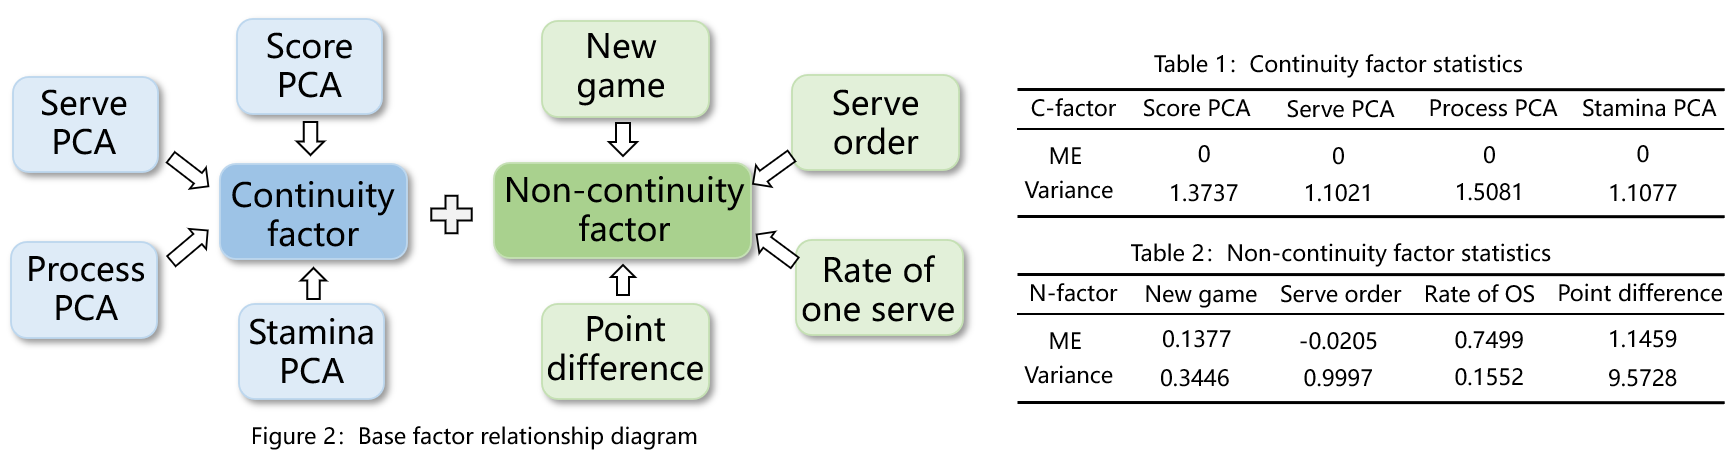
\includegraphics[width=15cm]{5.factor diagram}
\end{figure}

We conducted correlation tests on these eight dimensions to ensure the absence of multicollinearity, as shown in the results.

\begin{figure}[ht]%原来的
  \small
  \centering
  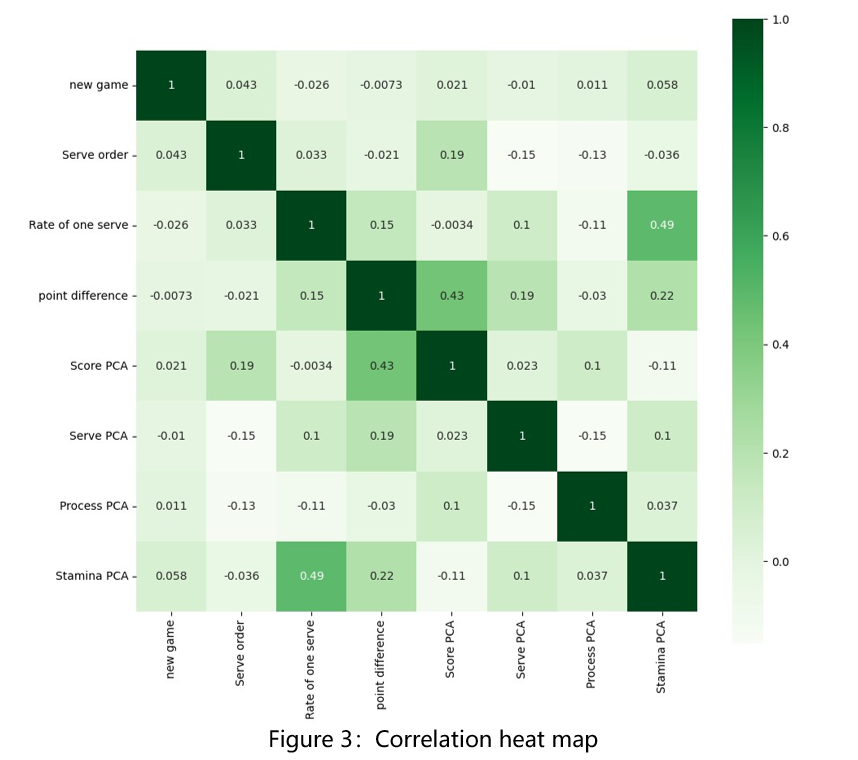
\includegraphics[width=11cm]{5.correlation test}
\end{figure}

Considering the higher-order effects of momentum and the interactions between factors, we included quadratic terms of continuous factors and interaction terms between continuous and non-continuous factors, resulting in a total of 28 feature vectors $(X_i$). These vectors were then subjected to logistic regression analysis using both the horseshoe prior Bayesian estimation method and traditional MLE methods.

\textbf{Model Result Interpretation}

Initially, we compared the coefficients estimated under the horseshoe prior and MLE for match ID-1071. 

\begin{figure}[ht]
  \small
  \centering
  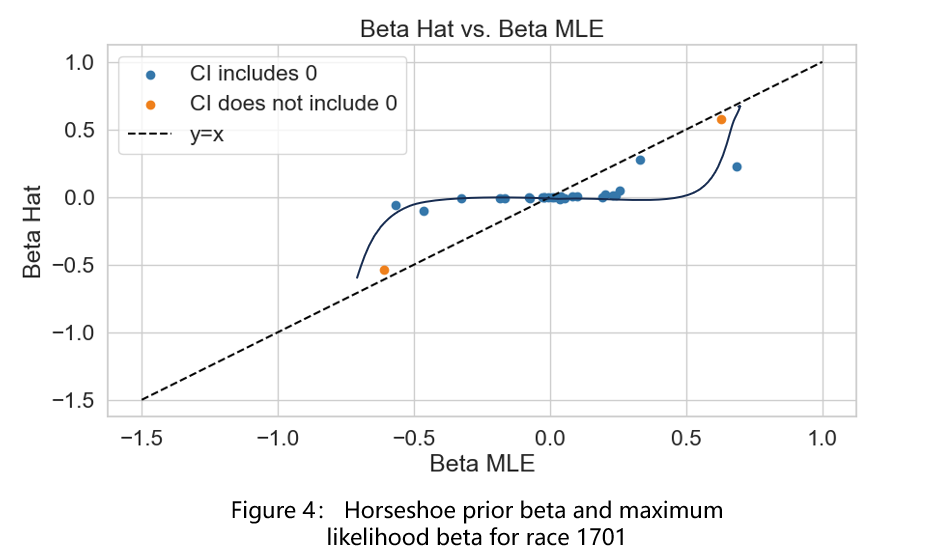
\includegraphics[width=10cm]{5.Comparison chart of MLE and Bayesian estimation}
\end{figure}

The results clearly demonstrated that for the majority of features, the horseshoe prior effectively shrinks their coefficients to zero, except where feature coefficients exhibited high credibility, which then approached the 45° line indicating lesser shrinkage. This finding underscores the sparsity of constructed features in tennis match predictions and how the horseshoe prior adeptly manages sparsity and noise to enhance model predictive accuracy.

Further, we compared the relative and absolute accuracies of the Bayesian estimates using the horseshoe prior and MLE across 31 matches.

\begin{figure}[ht]
  \centering
  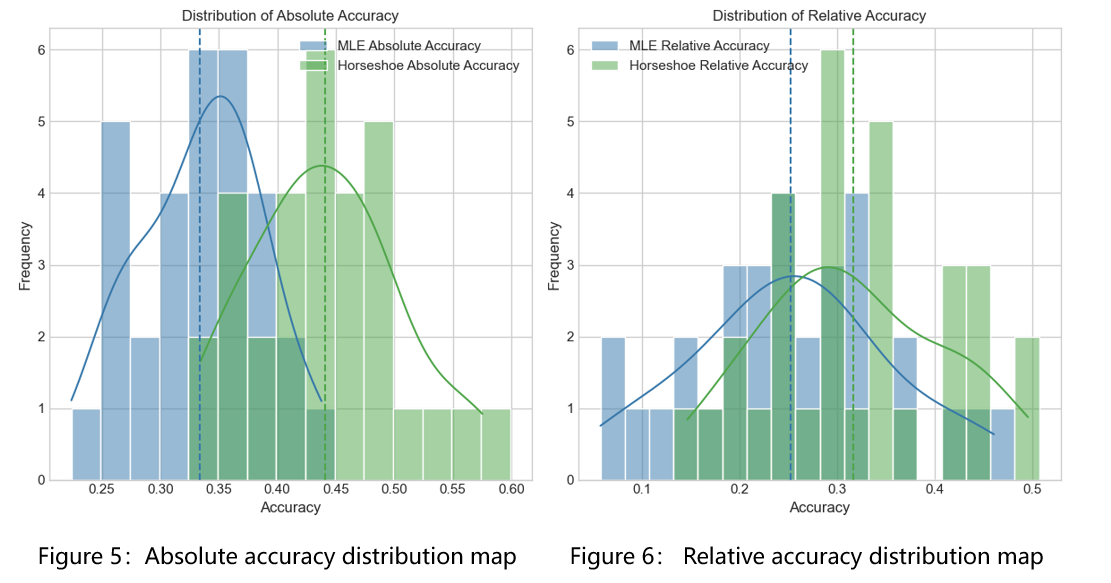
\includegraphics[width=13cm]{5.Accuracy distribution chart1}
\end{figure}

The results indicated that while the horseshoe prior generally outperformed MLE in terms of accuracy distributions, the overall improvements were modest. The effectiveness of the horseshoe prior in reducing irrelevant feature interference without diminishing model performance highlights its capability to focus on and utilize factors that significantly contribute to prediction outcomes. Additionally, this shrinkage effect aids in mitigating the risk of model overfitting, thereby enhancing the model's generalizability to unseen data. Despite limited overall accuracy improvements, the methodological superiority of this approach lies in providing decision-makers with more reliable and interpretative predictive model outcomes. This is particularly crucial in the context of sports competition predictions, where identifying and leveraging key information is essential for enhancing predictive accuracy, and the Bayesian logistic regression model with a horseshoe prior offers an efficient solution for such high-dimensional data environments.

\begin{figure}[ht]
  \centering
  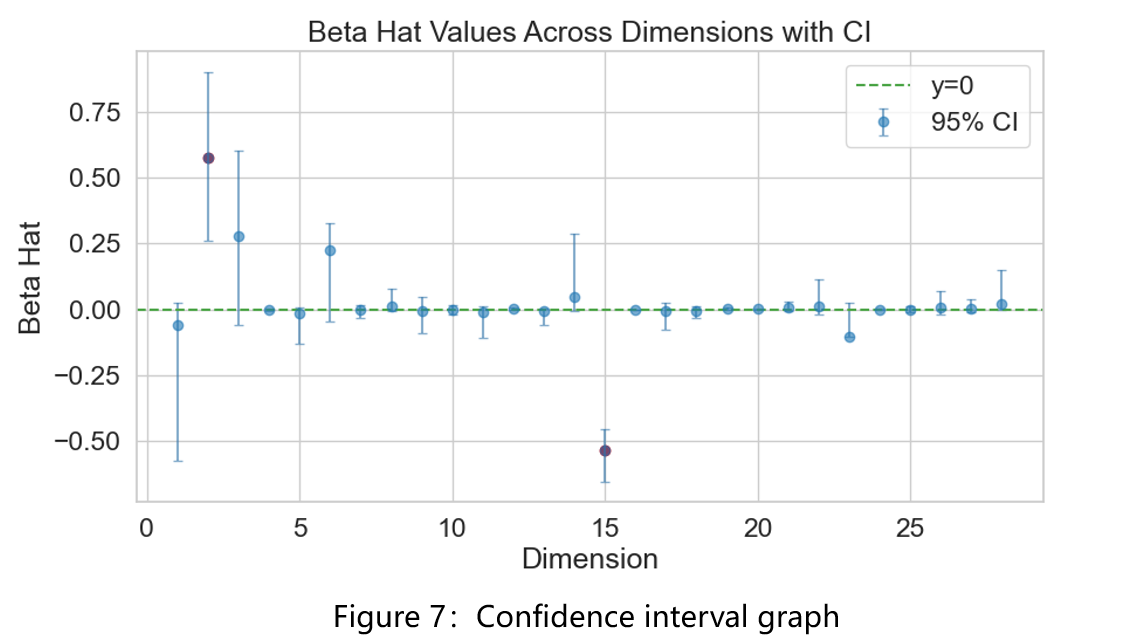
\includegraphics[width=10cm]{5.Confidence Interval}
\end{figure}

Figure 7 presents a key finding from the credible interval analysis for match ID-1071. Primarily, the coefficients for most features are significantly shrunk towards values close to zero, further affirming the sparsity of features in tennis match predictions. This sparsity suggests that although the model may contain a large number of potential predictive variables, only a few genuinely contribute substantially to predicting match outcomes. Notably, the "who serves" feature consistently showed significant predictive value across 27 matches, underscoring the advantage of the server in tennis and its significant impact on match outcomes. Besides, beyond the universally significant "who serves" feature, the significance of other features exhibited notable heterogeneity across different matches. This observation indicates that while certain factors may significantly influence the outcome in specific matches, their effects are not universally applicable across all matches. Therefore, the model must adapt to the unique circumstances of each match, flexibly identifying and utilizing those factors that are truly important for the given contest.

\textbf{Athlete Performance Evaluation}

We utilize the parameter $\sigma(\beta_0 + X_i^T\beta)$ from the likelihood $y_i | \beta, \beta_0 \sim \text{Bernoulli}\left(\sigma(\beta_0 + X_i^T\beta)\right)$, representing the win probability for player 1 in each round, as a metric to evaluate their performance quality. Given the unclear lag effect of our constructed indicators, we employed both cumulative time prediction and rolling time prediction methods to forecast the next three points for each dataset fitting. As illustrated in Figure 8 and Figure 9, the cumulative time prediction method demonstrates the long-term impact of momentum on win probabilities, whereas the rolling time prediction method highlights the influence of momentum on the win probability for imminent points. These time-series forecasting methods, by not utilizing future information for estimating a particular moment, align more closely with the natural progression of match outcomes.
\begin{figure}[ht]
  \small
  \centering
  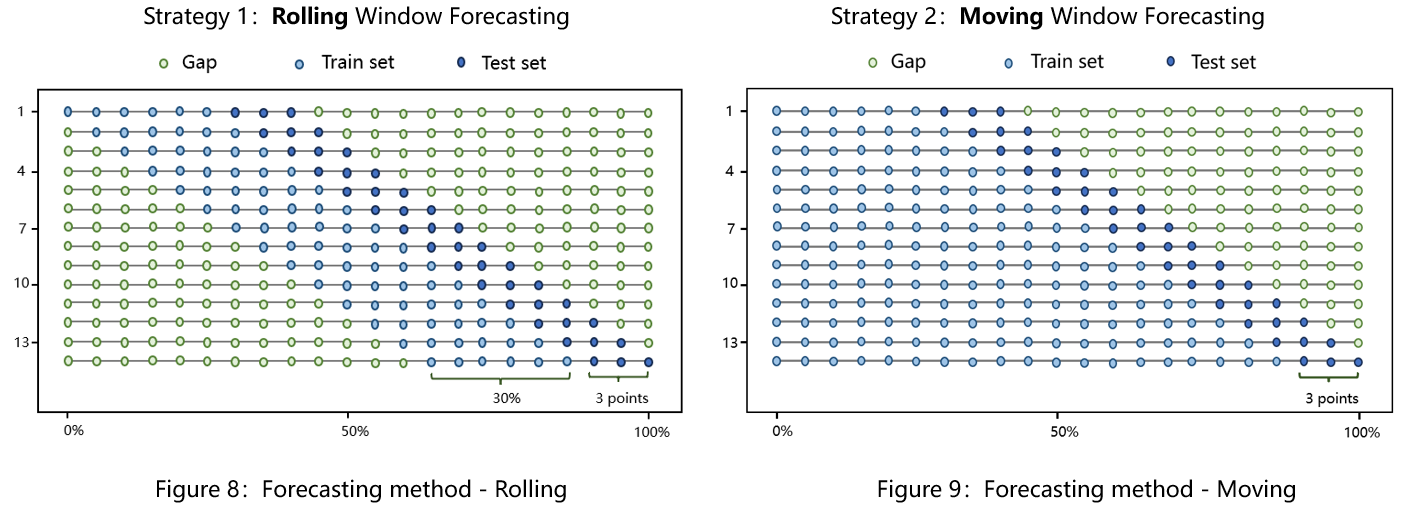
\includegraphics[width=16cm]{5.Strategy}
\end{figure}

For each strategy, we provided two accuracy metrics - absolute and relative accuracies - for the next three points using both maximum likelihood estimation and horseshoe prior estimation.The results are shown in the table below.
\begin{figure}[ht]
  \small
  \centering
  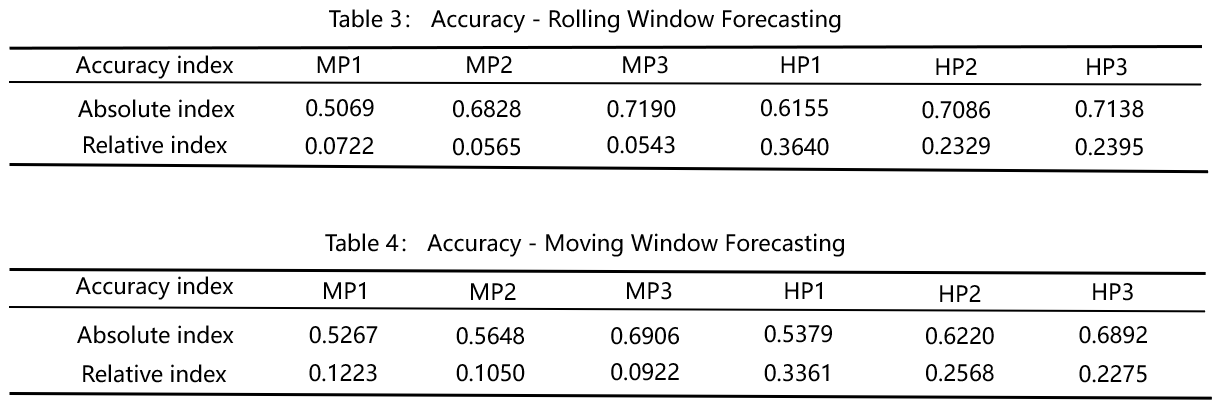
\includegraphics[width=12cm]{5.table}
\end{figure}

The comparison of these methods in the table reconfirms the superiority of the horseshoe prior over the MLE method, with the horseshoe prior method showing higher accuracy indicators for future rounds, regardless of whether it's moving window or rolling window predictions. The longitudinal comparison highlights that the prediction for future moments is more accurate than for the immediate next moment, indicating that the momentum features constructed by our method exhibit a certain degree of short-term lag. We noted that the moving method reflects the long-term impact of momentum, whereas the rolling method captures short-term effects. A vertical comparison of the two tables reveals that momentum's role is predominantly manifested in the short-term effects.

The highest accuracy point, the third one, under horseshoe prior estimation $\sigma(\beta_0 + X_i^T\beta)$, underwent a visualization of its parameter changes over time, as seen in Figures 10 and 11.
\begin{figure}[ht]%原来的
  \small
  \centering
  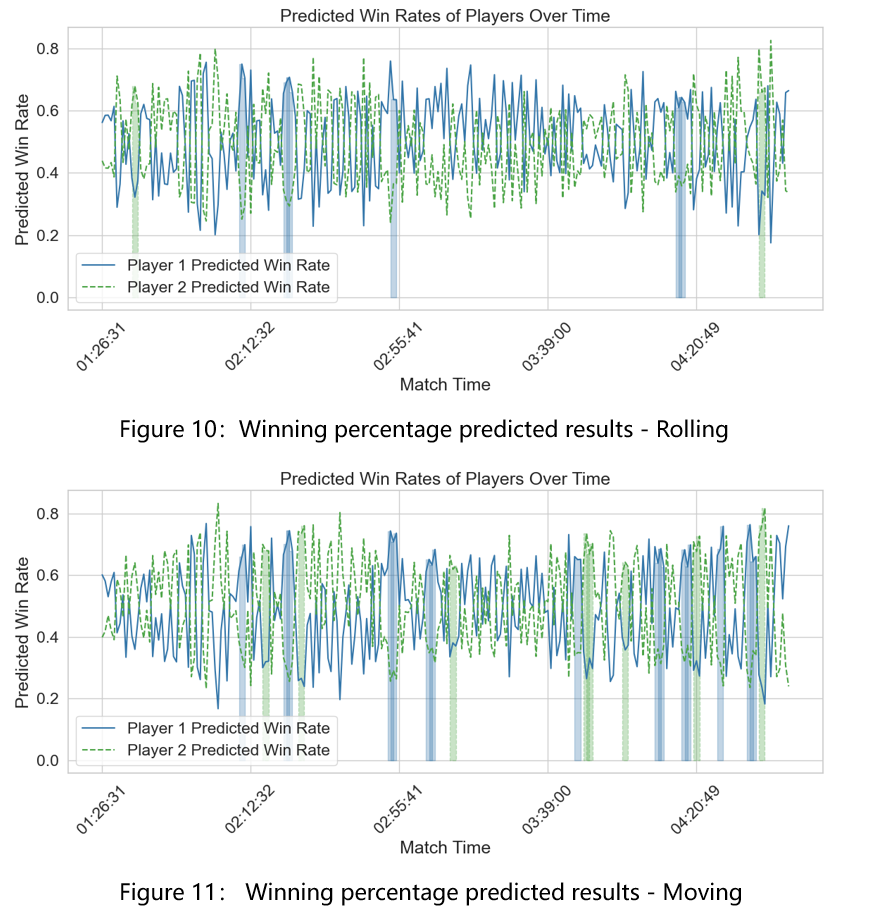
\includegraphics[width=13cm]{5.win_rate}
\end{figure}

We observed significant fluctuations and randomness in win probabilities, reflecting the inherent unpredictability of sports competitions. In both rolling and cumulative strategy predictions, the win probabilities fluctuated around the value of 0.5, further validating the randomness and sparsity of features involved in sports like tennis.

Under the rolling strategy, win probabilities were estimated based on short-term historical information, whereas, for the cumulative strategy, they were based on known long-term historical information. The prediction of continuous high win rates under both strategies showed differences, with continuous high win rates being notably less under the rolling strategy. This aligns with conventional wisdom that the more historical information we have, the more inclined we are to predict a stable win rate for a player. However, as indicated by previous accuracy results, the rolling strategy provides higher accuracy, suggesting that in sports competitions like tennis, short-term historical information has greater predictive value, and long-term historical information, if unverified, could potentially mislead our judgment.



\section{Problem 2: Momentum Model}

We compare the accuracy of a model with momentum-related factors removed against the original model to investigate the role of momentum in tennis matches. Further, by eliminating all indicators except the scoring information and establishing a Beta-Bernoulli model, we compare its accuracy with the original model to explore the randomness of outcomes in each round.

\subsection{Role of Momentum}

To assess whether momentum plays a role in match outcomes, we first assume that momentum does not influence the game. We remove all features related to momentum from Problem 1, retaining only six non-momentum indicators for match ID-1071, using a logistic regression model under horseshoe prior.

We compare the coefficients estimated under the horseshoe prior with those from the MLE method, also obtaining credible intervals. The analysis shows that among the four non-continuity factors, only the "who serves" feature is significant, while others are shrunk close to zero.

Upon refitting these models to 31 matches, we observe the distribution of both types of accuracies as follows:

\begin{figure}[ht]%原来的
  \small
  \centering
  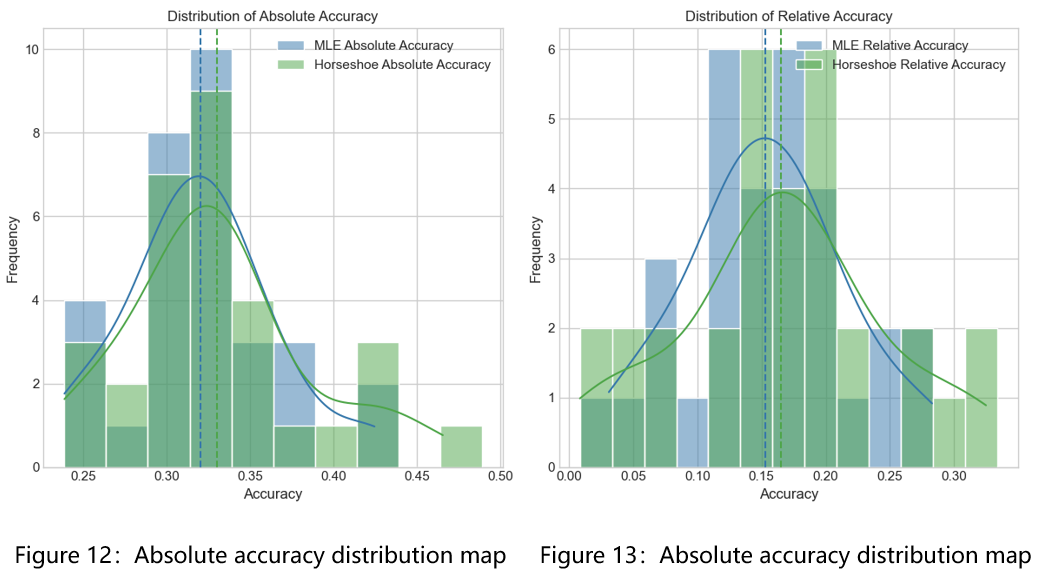
\includegraphics[width=13cm]{6.1accuracy}
\end{figure}

Figure 12 and Figure 13 reveal that, compared to models including momentum factors, the accuracy in predicting match outcomes slightly decreases when momentum is removed. The transition from high to low-dimensional features limits the enhancement potential of the Horseshoe Model. It is important to note that the addition of momentum factors is crucial for improving prediction accuracy. Even if we cannot identify a single highly effective momentum factor for predicting every match, by constructing a range of potential momentum factors and employing specific methods (e.g., Horseshoe), we can enhance the predictive accuracy.

\newpage
\subsection{Randomness of Winning}

Building on the "without momentum" basis to further confirm the volatility of performance and the randomness of winning, we established a baseline Beta-Bernoulli model. This model, focusing solely on the scoring process of the match, represents a scenario where winning is considered entirely random, offering greater randomness compared to the "without momentum" model.

\textbf{Establishment of the Baseline Model:}

The baseline model aims to solve the posterior distribution of $\theta_i$ given the sequence of wins and losses $y = (y_1, y_2, \ldots, y_n)$, employing Bayesian statistical methods. Here, $\theta_i$ represents the winning probability of player 1 in the $i$-th round, and $W_i | \theta_i \sim \text{Bern}(\theta_i)$ denotes the win-loss random variable for the $i$-th round.

\textbf{Model Assumptions:}

\begin{itemize}
  \item \textbf{Win-Loss Model:} In the $i$-th round, the victory of player 1 can be represented by a Bernoulli random variable $W_i$, where $W_i | \theta_i \sim \text{Bern}(\theta_i)$. This means if player 1 wins in the $i$-th round, then $W_i = 1$; otherwise, $W_i = 0$.
  \item \textbf{Prior Distribution of Winning Probability:} It is assumed that $\theta_i$ follows a $\text{Beta}(\alpha, \beta)$ distribution, which is concentrated around 0.5, indicating that, without any prior information, the probability of player 1 winning any round is equal. The Beta distribution is a continuous distribution defined in the [0, 1] interval, making it very suitable as a prior distribution for probabilities.
\end{itemize}

\textbf{Model Derivation:}


Given the sequence of win-loss outcomes $y = (y_1, y_2, \ldots, y_n)$, we aim to solve for the posterior distribution of $\theta_i$. Bayesian theorem provides a method to update the probability distribution of unknown parameters using prior knowledge and observed data. According to Bayesian theorem, the posterior distribution of $\theta_i$ can be calculated as follows:
$$
p(\theta_i | y) \propto p(y | \theta_i) p(\theta_i)
$$
where $p(y | \theta_i)$ is the likelihood function, and $p(\theta_i)$ is the prior distribution of $\theta_i$.

\begin{itemize}
\item \textbf{Likelihood Function:} Since $W_i | \theta_i \sim \text{Bern}(\theta_i)$, given $y_i$, the likelihood function for the $i$-th round is $\theta_i^{y_i} (1 - \theta_i)^{1 - y_i}$.
\item \textbf{Prior Distribution:} The prior distribution of $\theta_i$ is $\text{Beta}(\alpha, \beta)$, with the density function $p(\theta_i) = \frac{\theta_i^{\alpha-1} (1 - \theta_i)^{\beta-1}}{B(\alpha, \beta)}$, where $B(\alpha, \beta)$ is the Beta function.
\end{itemize}

Combining the likelihood function and the prior distribution, the posterior distribution of $\theta_i$ is:
$$
p(\theta_i | y) \propto \theta_i^{\alpha-1 + y_i} (1 - \theta_i)^{\beta-1 + 1 - y_i}
$$

Due to the conjugate relationship between the binomial distribution (a generalization of the Bernoulli distribution) and the beta distribution, the posterior distribution of $\theta_i | y$ is also identified as a beta distribution:
$$
\theta_i | y \sim \text{Beta}(\alpha + \sum_{j=1}^{i} y_j, \beta + i - \sum_{j=1}^{i} y_j)
$$

Next, we simulate the match with ID-1071, obtaining the following results, as shown in Figure 14. 
\begin{figure}[ht]%原来的
  \small
  \centering
  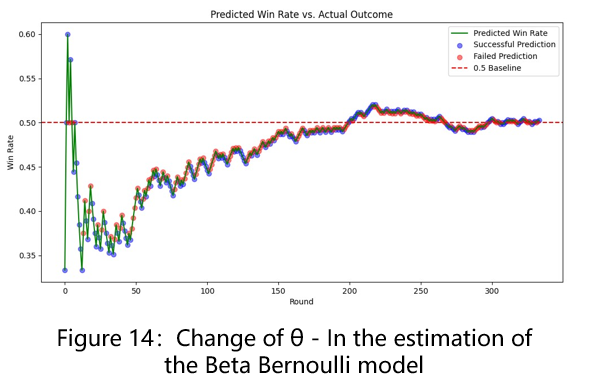
\includegraphics[width=11cm]{6.2predict win rate}
\end{figure}
The line represents $\theta_i$, the winning probability of player 1, with blue data points indicating successful predictions and red data points denoting failed predictions. This simulation shows low values for both relative and absolute accuracies, indicating that while our model can capture the trend of winning probabilities, its predictive power remains limited without considering additional information, especially the serving player factor.

Moreover, we observe that as the match progresses, the value of $\theta_i$ gradually trends towards 0.5, suggesting that without specific situational or influencing factors considered, the uncertainty of predictions increases over time.

A similar simulation analysis was conducted for the remaining 30 matches, and we found that in a total of 31 matches, $\theta_i$ for 24 matches showed a trend towards convergence at 0.5. This suggests that in most cases, as the match progresses, the winning probabilities of both players tend towards equality, reflecting a greater randomness in professional long-term matches when no additional information is provided. This reveals a certain degree of long-term unpredictability in sports competitions.

\section{Problem 3: Reversal Model}
\subsection{Problem 3.1: Factors Influencing Turning Points}

In matches, it's common to witness a change in momentum, often referred to as "reversal." To capture situations where a series of consecutive wins (or losses) is followed by a loss (or win), we identified three types of turning points: two consecutive points, three consecutive points, and four consecutive points. After extracting and fitting turning points, we found the fitting results for three consecutive points to be the most accurate. Considering that a reversal after two consecutive wins/losses is a common occurrence and may not necessarily indicate a change in momentum, and reversals after four consecutive wins/losses are less common and thus sparsely represented, we ultimately chose three consecutive points for our analysis.

We shifted our investigation from factors influencing fluctuations in matches to factors causing turning points. Utilizing the 28 features processed from the initial indicators in Problem 1, we extracted data for periods when turning points occurred and applied the horseshoe prior within a Bayesian logistic regression framework. Unlike previous models, this model calculates how each feature influences the probability of a reversal, rather than affecting the scoring probability.

For match ID-1701, using the same factors, we fit the model to determine the impact of each feature on the probability of a reversal.
\begin{figure}[ht]%原来的
  \small
  \centering
  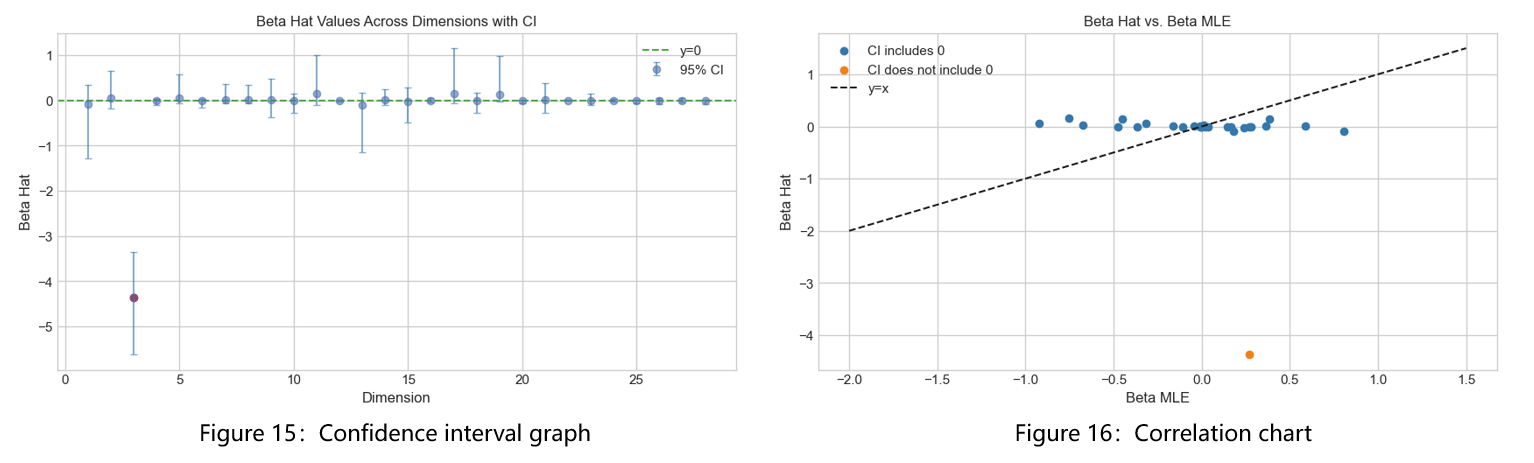
\includegraphics[width=17cm]{7.1 picture}
\end{figure}
It was observed that with the application of the horseshoe prior's shrinkage estimation, the majority of features were shrunk towards zero, indicating that, similar to match outcomes, features influencing reversals are sparse.

The only variable with high credibility for match ID-1701 was "first serve success rate." Similar estimations were made for the remaining 30 matches, where "first serve success rate" was found to be a significant factor in 29 matches.

This variable has a negative correlation with reversals, meaning that a higher proportion of successful first serves leads to fewer match reversals. This conclusion can be explained by several factors: a high first serve success rate objectively reflects a player's good performance in a match, increasing the likelihood of maintaining scoring opportunities and positive psychological effects, thus sustaining consecutive scores. However, a high first serve success rate might also mislead the trailing player into believing their scoring strategy is without fault, preventing strategy adjustments and leading to continued losses.

\begin{figure}[ht]%原来的
  \small
  \centering
  \includegraphics[width=13cm]{7.1 accuracy}
\end{figure}

The horseshoe prior's improvement in both absolute and relative accuracy over maximum likelihood estimation (MLE) further validates the significance of the "first serve success rate" factor in predicting match reversals. It also reaffirms the horseshoe prior's effectiveness in identifying key information amidst noisy, high-dimensional, sparse feature sets typical of tennis match predictions.

\subsection{Problem 3.2: Advice to Players}

As a professional data modeler and top-tier Bayesian statistician, it's crucial to recognize that each match represents a new beginning, where momentum might have short-term predictive value for outcomes. Regardless of performance in the previous round, past momentum becomes irrelevant in subsequent matches. Athletes should trust in their ability to turn the tide with positive adjustments if the previous match was lost or poorly played. Conversely, if a match was won by a large margin, it should not be assumed that this state will persist; maintaining composure is essential for continuing past momentum into future games.

Athletes must acknowledge the heterogeneity between past and upcoming matches, understanding that different matches may be influenced by various momentum factors. It's advisable to meticulously analyze opponents' performances under similar conditions to better anticipate potential trends, prepare mentally for unforeseen events, and minimize surprises. While other types of matches offer valuable insights, primarily in technical skills within tennis, the technical and momentum values provided by opponents' past match information should be distinctly recognized to gain an advantage in forthcoming games.

Flexibility in strategy is paramount. Perceived momentum can often be disrupted by unrelated factors. As a professional athlete, maintaining adaptability to adjust tactics based on the latest performance and characteristics of the opponent is crucial. Relying on long-term trends should be avoided in favor of tactical adjustments based on the current situation.

Moreover, considering the impact of momentum fluctuations, mental resilience becomes vital. Athletes should develop their capacity to handle pressure, adversity, and unexpected scenarios to ensure calmness and focus in future matches. Additionally, it's important to strategically utilize rules to disrupt the opponent's momentum without breaching professional ethics or competition regulations, thereby maximizing one's advantage.

\section{Problem 4: Model Generalization}

Our model employs both absolute and relative accuracy metrics to evaluate its effectiveness, which has been elaborated upon previously and will not be reiterated here.

To validate the generalizability of our model, we gathered data from women's tennis matches, men's tennis matches on different surfaces, and table tennis matches to predict win rates. Due to the relative difficulty in data collection and to mitigate the impact of missing indicators on prediction outcomes, we selected three matches with significant score differences to extract momentum factors for predictions.

\begin{figure}[ht]%原来的
  \small
  \centering
  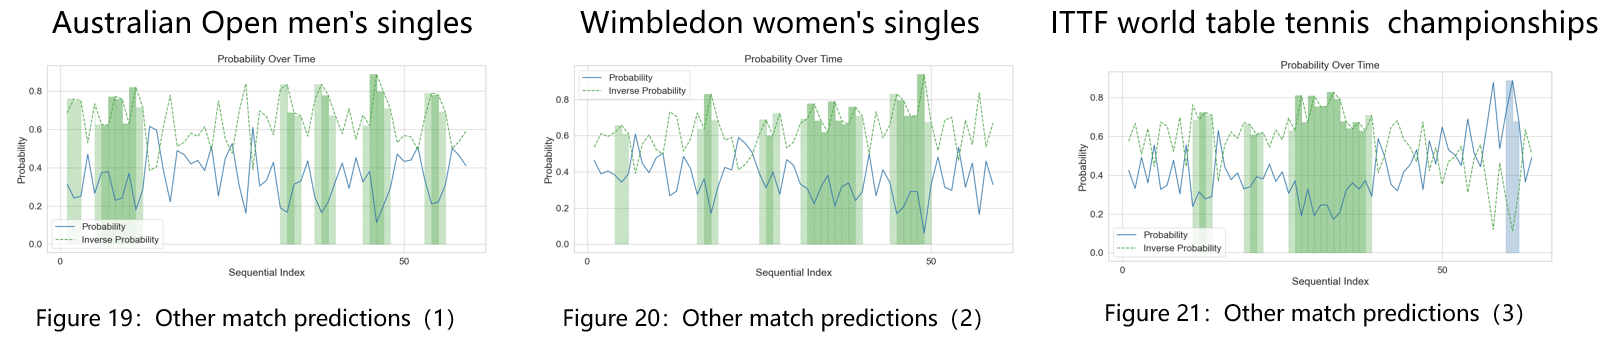
\includegraphics[width=16cm]{8.picture}
\end{figure}

For tennis matches in other categories, our model accurately predicted the direction of the match. This indicates that the model has a strong predictive capability for tennis matches with a clear winner, effectively interpreting the role of momentum. However, for table tennis matches, although initial model predictions aligned with the early stages of the match, predictions for the mid to late stages were inaccurate. This discrepancy may be attributed to the model's imprecise extraction of momentum factors specific to table tennis. It is evident that for different sports, provided that relatively complete and informative momentum factors are extracted, the model demonstrates robust predictive performance.

\section{Strengths and Weaknesses of Our Strategy}


The Horseshoe prior-based logistic regression model excels in identifying critical factors from high-dimensional and noisy data, improving both absolute and relative accuracy of predicting match win rates and reversal occurrences over maximum likelihood estimation. Benefiting from the inherent advantages of Bayesian statistics, our model is applicable even in matches with fewer rounds, as it is not constrained by large sample assumptions. However, the model is limited to dealing with the high-dimensional feature impacts within a single match and cannot perform personalized modeling for each player involved in the match. Moreover, our model relies on time-window forecasting to handle factors that change over time within the same match, which increases computational time.Specifically, due to the complex sampling calculations required for Bayesian posterior distribution estimation, multiple fittings for the same match result in our model requiring several hours per single time-window strategy, posing a challenge for real-time analysis and deployment.

\section{Conclusion}

In professional tennis matches, the win probability for each point exhibits significant \textbf{randomness} and \textbf{volatility}. Posterior estimates based solely on historical match outcomes tend to \textbf{converge towards 0.5}, indicating a degree of \textbf{unpredictability} in match results. Nevertheless, incorporating potential momentum and additional historical information remains \textbf{effect}. Despite the challenges posed by \textbf{high-dimensional} and \textbf{sparse} feature spaces, applying \textbf{noise-handling techniques} such as the \textbf{horseshoe prior} allows for the selection of \textbf{credible} factors that hold predictive value for future matches. 

When employing \textbf{Bayesian logistic regression} models for rolling predictions, the use of long-term historical information tends to \textbf{stabilize predictions}. However, it has been observed that short-term historical data carry greater predictive value in sports such as tennis, where long-term information may be \textbf{misleading} due to \textbf{noise contamination}. Moreover, the significant \textbf{heterogeneity} observed in the majority of match features suggests that momentum factors vary across different matches, presenting challenges for data collection, noise reduction, and the widespread application of predictive models.

Predictions regarding point \textbf{reversals} in matches, while also characterized by high randomness and volatility, demonstrate a notable improvement in predictive accuracy when the model precisely addresses noise and sparsity issues. This contrasts with the stronger unpredictability associated with individual point win predictions.

In summary, our model demonstrates good adaptability when \textbf{generalized} to other types of matches, owing to its capability to handle \textbf{high-dimensional} data and effectively \textbf{manage noise}. For matches with discernible trends, our model adeptly captures these patterns using historical data, thereby providing deeper insights for athletes, coaches, and sports analysts. These insights not only enhance the understanding of the inherent dynamics within competitive sports but may also support the modernization of sports training, strategy development, and match analysis.

\newpage
\section{Memorandum}

%下面是信件的格式不要随便改,会越改越丑的。。。。
\noindent\rule{\textwidth}{1pt}

\vspace{-0.2cm}

\noindent \ To: tennis coaches

\vspace{-0.2cm}

\noindent \ From: Team \#2412216 of 2024 MCM

\vspace{-0.2cm}

\noindent \ Date: February 6, 2024


\vspace{-0.4cm}

\noindent\rule{\textwidth}{1pt}

It is a common assumption that momentum plays a pivotal role in high-level competitive sports. However, after engaging with this modeling study, one might question the steadfastness of this belief.

We offer the following advice \textbf{to coaches}:

Understanding Unpredictability: As a coach, you should recognize the unpredictability of match outcomes. Many uncontrollable factors can influence a match's result, and it is essential to incorporate this uncertainty into your tactical planning. Additionally, try to leverage certain potential momentum factors in your strategies to secure an advantage for your players.

Observation and Emotional Stability: Tennis matches are lengthy battles where momentum, as a short-term factor, seldom determines the final outcome. Temporary advantages or disadvantages do not dictate the direction of the match. As a coach, you should assist your players in managing their emotions: remain vigilant during winning streaks and composed during losses.

Acknowledging Heterogeneity: Be aware of the heterogeneity in sports competitions; momentum factors can significantly vary between matches. This implies that athletes should never underestimate their opponents, even if they have won against them in the past. Stay attuned to the nuances of each match, ready to tackle specific situations and adjust to changes. Analyzing opponents' strengths and weaknesses, and adjusting strategies accordingly, is crucial for securing victories. Sometimes, strategies that worked in the past may not be effective in future matches. Identifying opponents' vulnerabilities, such as a weakness for high balls, and crafting tailored strategies can be instrumental. Observing opponents' playing styles and technical characteristics throughout the match can provide insights into their tactical approaches, enabling timely and effective counter-strategies.

\textbf{To athletes}, we say:

The impact of momentum can be both significant and negligible. A tennis match can present various unforeseen situations: tension from an opponent's comeback, frustration from unforced errors, or despair from being a point away from defeat. We hope that after reading this memorandum, you reassure yourself that the concept of momentum pales in comparison to the success brought about by your hard work and dedication to the game. Trust in yourself and persevere in the matches ahead!

\vspace{\parskip}

Sincerely yours,

Your friends

\newpage
%后面的参考文献
\begin{thebibliography}{99}
\bibitem{1} Heston, L. S., Jones, S. C., Khorram, M., Option Momentum[J].The Journal of Finance,2023,78(6):3141-3192.
\bibitem{2} Asness, S. C., Moskwitz, J. T., Pedersen, H. L., Value and Momentum Everywhere[J].The Journal of Finance,2013,68(3):929-985.Addison-Wesley Publishing Company, 1986.
\bibitem{3} Rivera, J. (2023), Tennis scoring, explained: A guide to understanding the rules terms and point system at Wimbledon[DB/OL], The Sporting News.
\bibitem{4} Higham, A.(2000), Momentum - The Hidden Force in Tennis[M].
\bibitem{5} Gregory M. S., Johnathon L. D., Gerardo O. G. Winning and losing streaks in the National Hockey League : are teams experiencing momentum or are games a sequence of random events ? J. Quant. Anal. Sports 2021;17(3):155-170.
\bibitem{6} Moss and Donoghue O., Momentum in US Open men' s singles tennis[J]. International Journal of Performance Analysis in Sport,2015,15(3),884-896.
\bibitem{7} Braidwood, J. (2023), Novak Djokovic has created a unique rival – is Wimbledon defeat the beginning of the end, The Independent[DB/OL].
\bibitem{8} Meier P ,Flepp R ,Ruedisser M , et al.Separating psychological momentum from strategic momentum: Evidence from men’s professional tennis[J].Journal of Economic Psychology,2020,78(prepublish):
\bibitem{9} Carvalho, Carlos M. et al. “Handling Sparsity via the Horseshoe.” International Conference on Artificial Intelligence and Statistics (2009).
\bibitem{10} Enes Makalic,and Daniel F. Schmidt.A Simple Sampler for the Horseshoe Estimator..IEEE Signal Process. Lett. 23.1(2016):179-182.
\bibitem{11} 2024 Australian Open men's singles semifinal: Novak DJOKOVIC against Jannik SINNER[DB/OL].
\bibitem{12} 2023 Wimbledon women's singles final Marketa: VONDROUSOVA versus Ons JABEUR[DB/OL].
\bibitem{13} 2023 WTT men's singles semifinal: Ma Long against Wang Chuqin[DB/OL].
\end{thebibliography}

\newpage
\begin{appendices}

\textbf{Appendix A: Mathematical derivation}%这里是附录

This appendix provides a detailed mathematical derivation of the horseshoe prior in Bayesian logistic regression, including the establishment of the model, the derivation of the posterior distribution, and the method of parameter sampling.

\centerline{\textbf{Probabilistic Model Expression of Horseshoe Prior}}

Consider the Bayesian linear regression model, whose likelihood function is:
\begin{equation}
  y|X, \beta, \sigma^2 \sim \mathcal{N}_n(X\beta, \sigma^2 I_n)
  \tag{1}
\end{equation}
Here, $y \in \mathbb{R}^n$ is the response variable, $X \in \mathbb{R}^{n \times p}$ is the predictor variable matrix, $\beta \in \mathbb{R}^p$ is the coefficient vector, and $\sigma^2$ is the error variance.

\noindent\textbf{Construction of the Horseshoe Prior}

For the coefficient $\beta_j$, we introduce local shrinkage parameter $\lambda_j^2$ and global shrinkage parameter $\tau^2$, with prior distributions given by:
\begin{equation}
  \beta_j | \lambda^2_j, \tau^2, \sigma^2 \sim \mathcal{N}(0, \lambda_j^2 \tau^2 \sigma^2) \tag{2}
\end{equation}
\begin{equation}
  \lambda_j \sim C^+(0, 1) \tag{3}
\end{equation}
\begin{equation}
  \tau \sim C^+(0, 1)  \tag{4}
\end{equation}
Here, $C^+(0, 1)$ represents the standard half-Cauchy distribution.

\noindent\textbf{Posterior Distribution}

The derivation of the posterior distribution involves combining the likelihood function with the prior distribution and utilizing Bayes' theorem. Since direct computation of the posterior distribution is often infeasible, we introduce auxiliary variables $a$ and $x$ to simplify the calculations:
\begin{equation}
  x^2|a \sim IG(1/2, 1/a), \quad a \sim IG(1/2, 1/A^2) \tag{5}
\end{equation}
Let $x \sim C^+(0, A)$. Using this scale mixture representation, we introduce auxiliary variables $\nu_j$ and $\xi$ for each $\lambda_j^2$ and $\tau^2$:
\begin{equation}
  \lambda_j^2|\nu_j \sim IG(1/2, 1/\nu_j), \quad \nu_j \sim IG(1/2, 1) \tag{6}
\end{equation}
\begin{equation}
  \tau^2|\xi \sim IG(1/2, 1/\xi), \quad \xi \sim IG(1/2, 1) \tag{7}
\end{equation}

\noindent\textbf{Conditional Posterior Distribution of Parameters}

Using the auxiliary variables, the conditional posterior distribution of the coefficients $\beta$ is:
\begin{equation}
  \beta|\cdot \sim \mathcal{N}_p(\hat{\beta}, \hat{\Sigma}) \tag{8}
\end{equation}
where,
\begin{equation}
  \hat{\Sigma} = (\sigma^{-2}X^TX + D^{-1})^{-1}, \quad D = \text{diag}(\lambda_1^2\tau^2, \ldots, \lambda_p^2\tau^2) \tag{9}
\end{equation}
\begin{equation}
  \hat{\beta} = \hat{\Sigma}\sigma^{-2}X^Ty \tag{10}
\end{equation}
The conditional posterior distribution of $\sigma^2$ is an inverse gamma distribution: 
\begin{equation}
  \sigma^2|\cdot \sim IG\left(\alpha_n, \beta_n\right) \tag{11}
\end{equation}
Wherein, $\alpha_n$ and $\beta_n$ are updated based on the data and prior parameters.

The updating of local shrinkage parameter $\lambda_j^2$ and global shrinkage parameter $\tau^2$ depend on their corresponding auxiliary variables $\nu_j$ and $\xi$, enabling the entire sampling process to be implemented through the Gibbs sampling algorithm.

\centerline{\textbf{Posterior Distribution Sampling Method using Auxiliary Variables}}

\noindent\textbf{Pólya-gamma Data Augmentation Method}

For a logistic regression model, the relationship between the response variable $y_i \in \{0, 1\}$ and the predictor variable $\mathbf{x}_i$ is modeled using the logistic function, where $\psi_i = \beta_0 + \mathbf{x}_i^T \beta$ represents the log odds of success. In the Pólya-gamma data augmentation framework, we introduce auxiliary variables $\omega_i$, and for each observation $i$, the distribution of $\omega_i$ is defined as the Pólya-gamma distribution $PG(1, \psi_i)$.

\noindent\textbf{Sampling process}

1. Updating the auxiliary variable $\omega$: For each observation $i$, the conditional posterior distribution of $\omega_i$ is:
$$
  \omega_i | \beta, \beta_0, \mathbf{x}_i, y_i \sim PG(1, \psi_i)
$$
Wherein,$\psi_i = \beta_0 + \mathbf{x}_i^T \beta$.

2. Updating the coefficients $\beta$ and intercept $\beta_0$: Given the auxiliary variable $\omega_i$, the conditional posterior distribution of $\beta$ and $\beta_0$ can be expressed as a multivariate normal distribution, which takes the form:
$$
\beta | \cdot \sim \mathcal{N}(\mu_{\beta}, \Sigma_{\beta})
$$
Wherein,
$$
\Sigma_{\beta} = \left(X^T \Omega X + D^{-1}\right)^{-1},\quad \mu_{\beta} = \Sigma_{\beta} X^T \Omega \mathbf{z},
$$
$$
\Omega = \text{diag}(\omega_1, \ldots, \omega_n),\quad \mathbf{z} = X\beta + (\mathbf{y} - \frac{1}{2})/\omega,
$$
$D = \text{diag}(\lambda_1^2 \tau^2, \ldots, \lambda_p^2 \tau^2)$ is a diagonal matrix with shrunken parameters.

3. Updating the local shrinkage parameter $\lambda_j^2$: The conditional posterior distribution of the local shrinkage parameter $\lambda_j^2$ is an inverse gamma distribution, and the update formula is:
$$
\lambda_j^2 | \cdot \sim IG\left(\alpha_{\lambda}, \beta_{\lambda_j}\right)
$$
Wherein,
$$
\alpha_{\lambda} = 1 + \frac{1}{2}, \quad \beta_{\lambda_j} = \frac{1}{\nu_j} + \frac{\beta_j^2}{2 \tau^2}.
$$
4. Updating the global shrinkage parameter $\tau^2$: The conditional posterior distribution of the global shrinkage parameter $\tau^2$ is also an inverse gamma distribution, and the update formula is:
$$
\tau^2 | \cdot \sim IG\left(\alpha_{\tau} \beta_{\tau}\right)
$$
Wherein,
$$
\alpha_{\tau} = \frac{p + 1}{2},\quad \beta_{\tau} = \frac{1}{\xi} + \frac{1}{2} \sum_{j=1}^p \frac{\beta_j^2}{\lambda_j^2}.
$$
5. Updating the auxiliary variables $\nu_j$ and $\xi$: The conditional posterior distribution of the auxiliary variables is an inverse gamma distribution, and the update formula is:
$$
\nu_j | \cdot \sim IG\left(1, 1 + \frac{1}{\lambda_j^2}\right),\quad \xi | \cdot \sim IG\left(1, 1 + \frac{1}{\tau^2}\right).
$$
Repeat the above process until convergence or until the iteration count reaches the threshold.

\textbf{Appendix B: Program code}


\begin{figure}[ht]%原来的
  \small
  \centering
  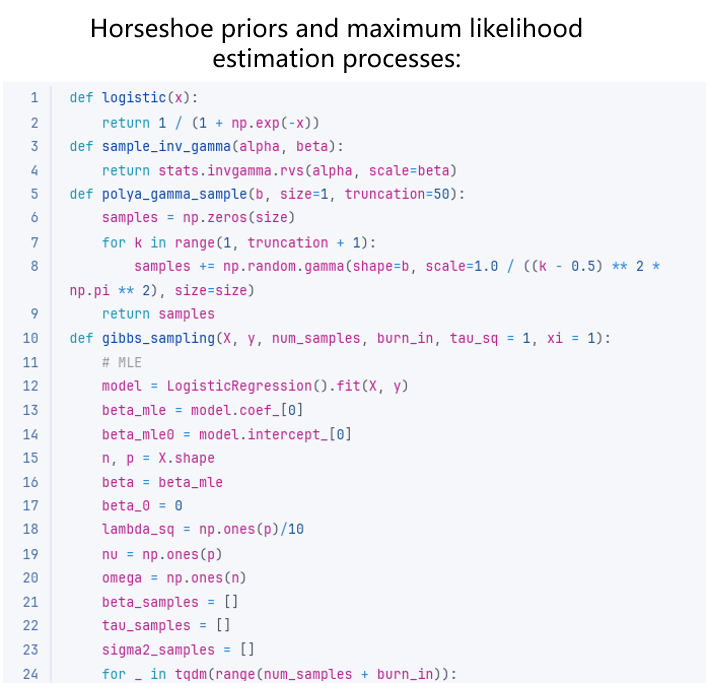
\includegraphics[width=16cm]{daima5}
\end{figure}

\begin{figure}[ht]%原来的
  \small
  \centering
  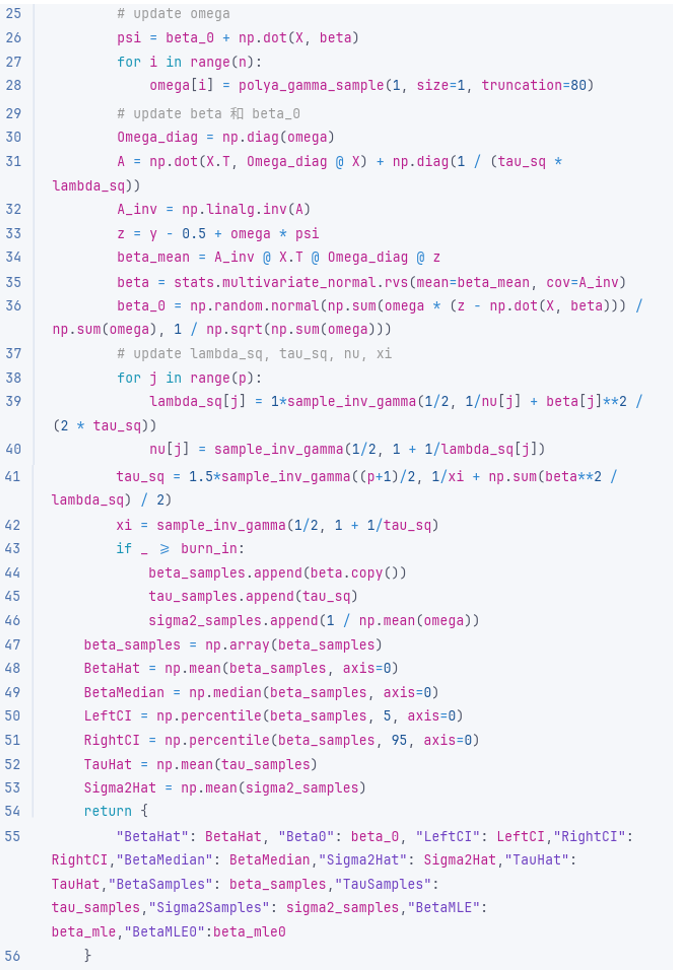
\includegraphics[width=16cm]{daima6}
\end{figure}

\begin{figure}[t]%原来的
  \small
  \centering
  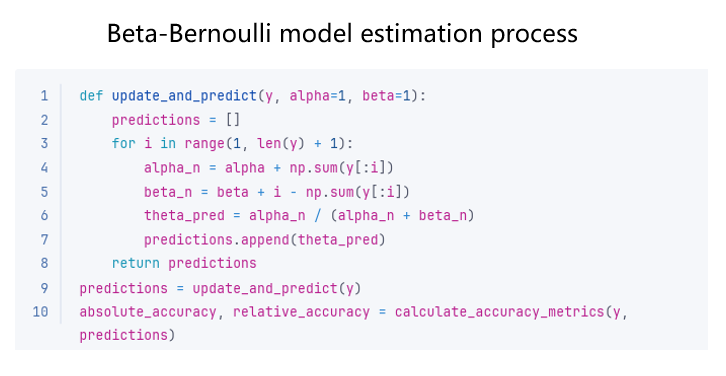
\includegraphics[width=16cm]{daima7}
\end{figure}

\end{appendices}
\end{document}
%% 
%% This work consists of these files mcmthesis.dtx,
%%                                   figures/ and
%%                                   code/,
%% and the derived files             mcmthesis.cls,
%%                                   mcmthesis-demo.tex,
%%                                   README,
%%                                   LICENSE,
%%                                   mcmthesis.pdf and
%%                                   mcmthesis-demo.pdf.
%%
%% End of file `mcmthesis-demo.tex'.
